\begin{activite}[Un pas de côté]

Cinq élèves ont construit une image du danseur, en effectuant chacun une translation différente :
\begin{enumerate}
 \item Sarah, de 5 cm dans la direction de $d$ ;
 \item Vincent, horizontalement, vers la droite ;
 \item Mélanie, selon le vecteur $\vec{c}$ ;
 \item Juan, en la glissant de 3 cm ;
 \item Madina, en la déplaçant de 4 cm, vers la gauche et dans la direction de $b$.
 \end{enumerate}
 \begin{minipage}[c]{0.58\linewidth}
  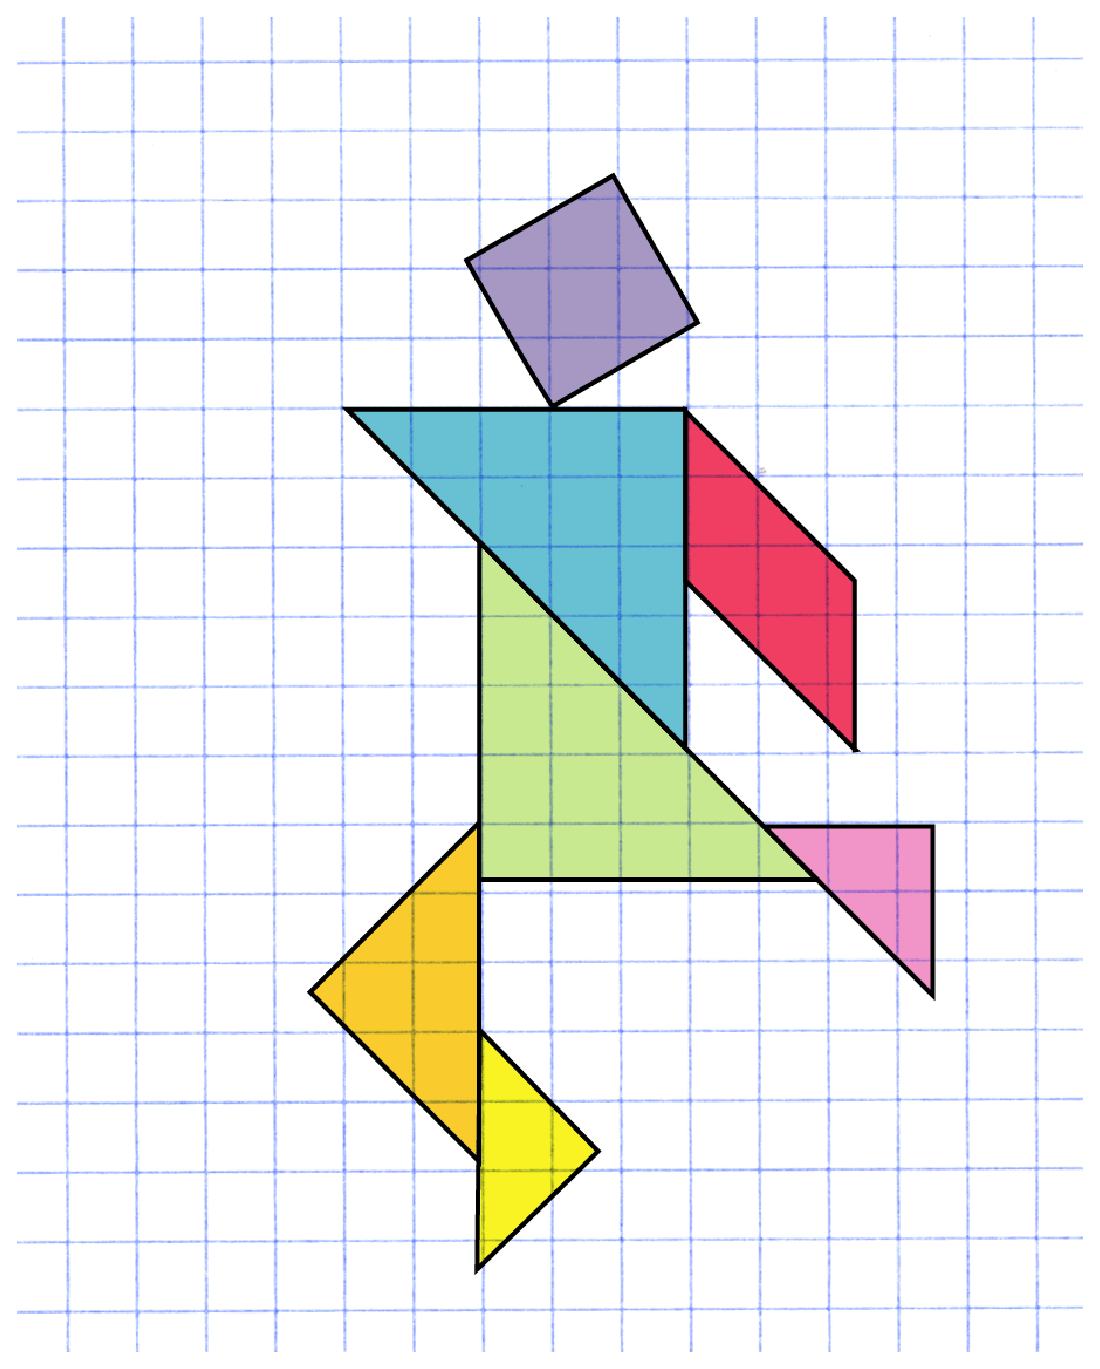
\includegraphics[width=8.4cm]{grille_danseur} 
  \end{minipage} \hfill%
  \begin{minipage}[c]{0.28\linewidth}
  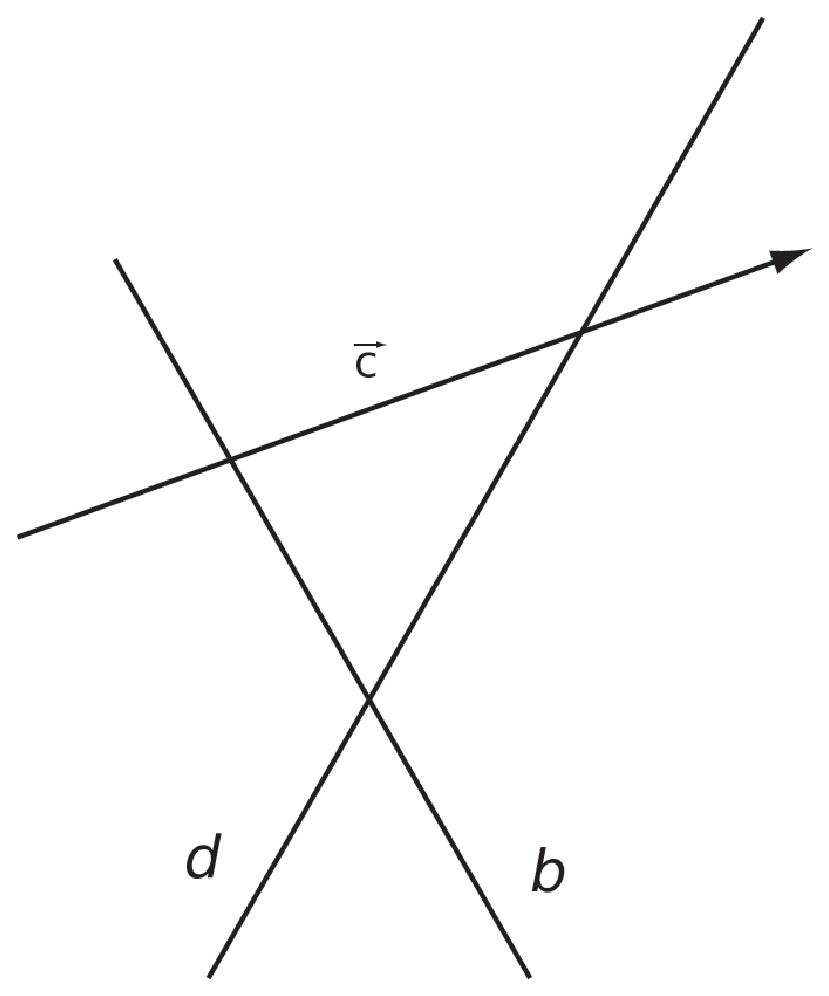
\includegraphics[width=4.2cm]{vecC_db}
  \end{minipage} \\
À l'aide des carreaux, construis ces cinq figures et compare tes résultats avec ceux de tes camarades.

\end{activite}

%%%%%%%%%%%%%%%%%%%%%%%%%%%%%%%%%%%%%%%%%%%%%%%%%%%%%%%%%%%%%%%%%%%%%%

%%%%%%%%%%%%%%%%%%%%%%%%%%%%%%%%%%%
%%%%%%%%%%%%%%%%%%%%%%%%%%%%%%%%%%%
%MiseEnPage
%%%%%%%%%%%%%%%%%%%%%%%%%%%%%%%%%%%
\newpage
%%%%%%%%%%%%%%%%%%%%%%%%%%%%%%%%%%%
%%%%%%%%%%%%%%%%%%%%%%%%%%%%%%%%%%%

\begin{activite}[Avoir du bons sens]

Voici une vingtaine de flèches représentant des vecteurs :
\begin{center} 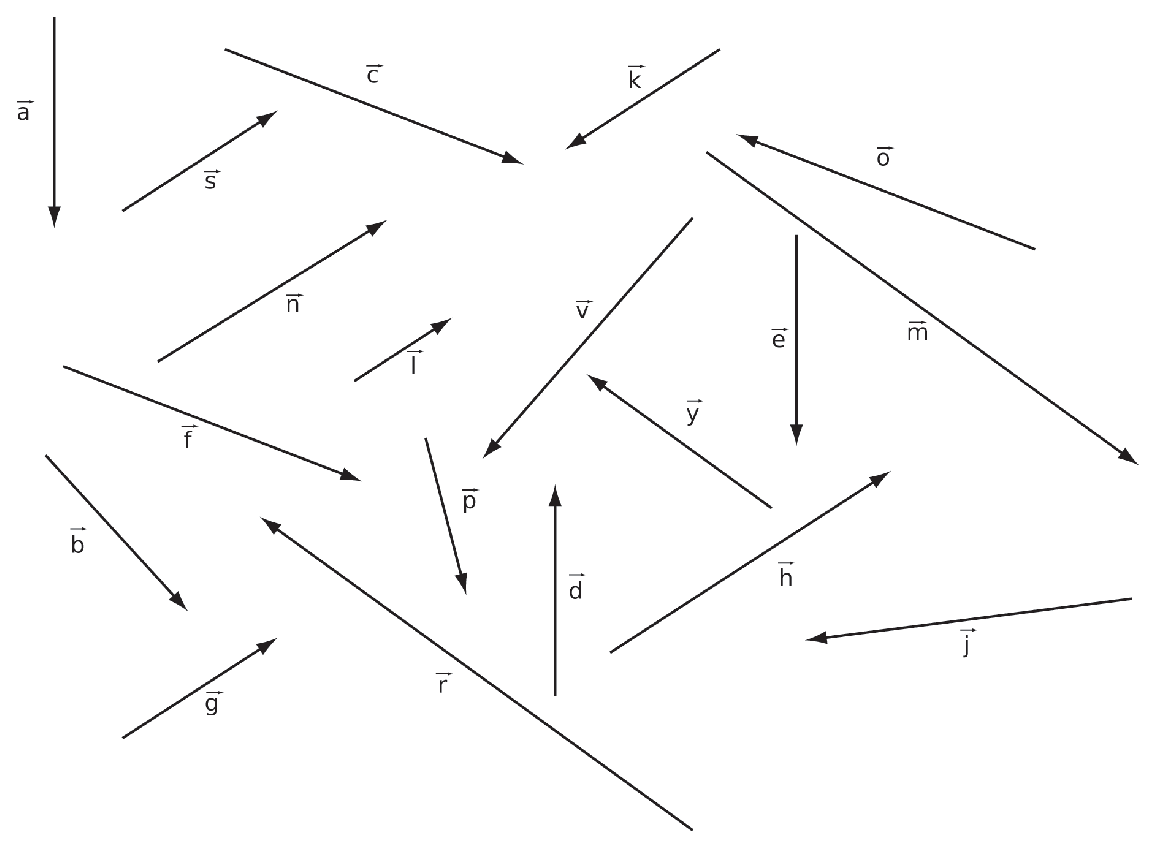
\includegraphics[width=16cm]{fleches_vecteurs}\end{center}

\begin{partie}[Classification]
Recopie puis complète le tableau en donnant tous les vecteurs possibles pour chaque question. Arrondis au dixième le plus proche tes mesures.
\begin{center}
 \renewcommand*\tabularxcolumn[1]{>{\centering\arraybackslash}m{#1}}
 \begin{ttableau}{0.9\linewidth}{4}
 \hline
 \rowcolor{A3}Vecteur & Même longueur que le vecteur & Même direction que le vecteur & Égal au vecteur \\\hline
 \rowcolor{F3} $\vec{a}$ & & & \\\hline
 \rowcolor{F3} $\vec{c}$ & & & \\\hline
 \rowcolor{F3} $\vec{q}$ & & & \\\hline
 \rowcolor{F3} $\vec{r}$ & & & \\\hline
 \end{ttableau}
 \end{center}
\end{partie}

\vspace{1em}

\begin{partie}[Qu'en penses-tu ?]
Détermine si les affirmations des élèves sont correctes ou non :
\begin{enumerate}
 \item Aline dit que le vecteur $\vec{c}$ est égal à deux fois le vecteur $\vec{a}$ ;
 \item Simon dit que le vecteur $\vec{d}$ est l'opposé du vecteur $\vec{e}$ ;
 \item Justine prétend que le vecteur $\vec{b}$ et $\vec{f}$ ont la même direction ;
 \item Mohamed dit que les vecteurs $\vec{c}$ et $\vec{j}$ ont la même intensité.
 \end{enumerate}
\end{partie}

\end{activite}

%%%%%%%%%%%%%%%%%%%%%%%%%%%%%%%%%%%%%%%%%%%%%%%%%%%%%%%%%%%%%%%%%%%%%%

\begin{activite}[Tourner dans tous les sens]

\begin{partie}[Dans quel sens]
 \begin{minipage}[c]{0.68\linewidth}
La figure ci-contre illustre une montre possédant qu'une seule aiguille.
\begin{enumerate}
 \item Reproduis le dessin puis dessine l'aiguille quand elle aura tourné de $90^\circ$ par rapport au centre $O$ ;
 \item Dessine l'aiguille quand elle aura tourné de $- 120^\circ$ par rapport au centre $O$.
 \end{enumerate}
  \end{minipage} \hfill%
  \begin{minipage}[c]{0.28\linewidth}
  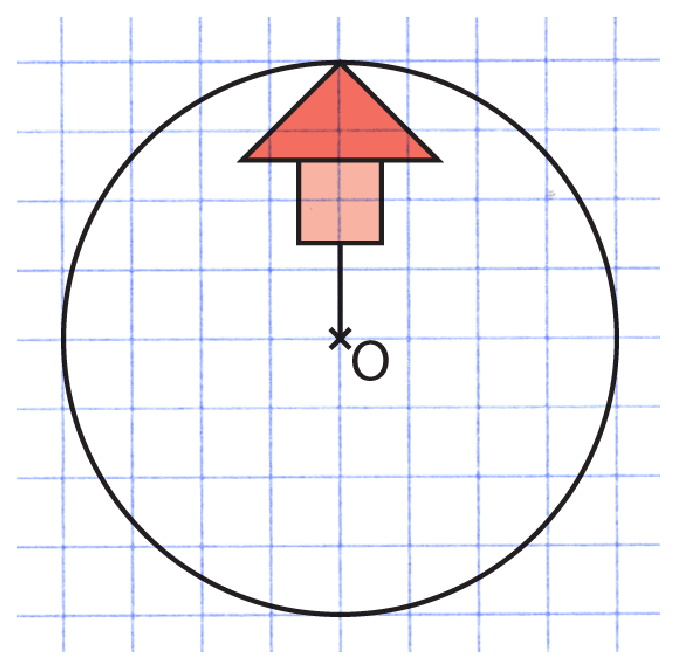
\includegraphics[width=4cm]{une_aiguille}
  \end{minipage} \\ 
\end{partie}

\begin{partie}[Le virage]
 \begin{minipage}[c]{0.50\linewidth}
Ci-contre une partie du circuit de Catalogne où la formule 1 vient d'entamer son virage.
\begin{enumerate}
 \item À l'aide d'un papier calque reproduit cette figure et dessine la voiture après qu'elle ait effectué une rotation de $80^\circ$ par rapport au centre $P$.
 \item Peut-on effectuer tout le virage en gardant le même rayon de rotation ?
 \end{enumerate}
  \end{minipage} \hfill%
  \begin{minipage}[c]{0.46\linewidth}
  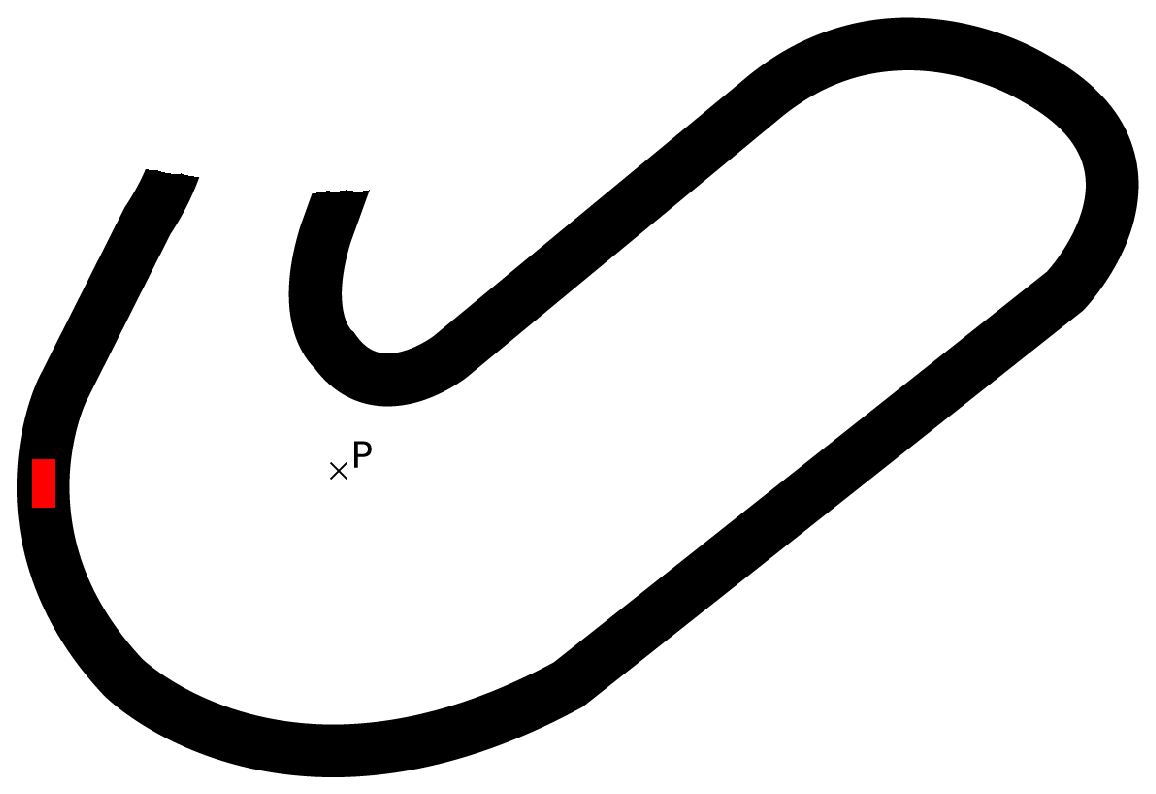
\includegraphics[width=6.9cm]{formule1_Catalogne}
  \end{minipage} \\ 
\end{partie}

\begin{partie}[Trouver le centre]
\vspace{.5em}
 \begin{minipage}[c]{0.28\linewidth}
  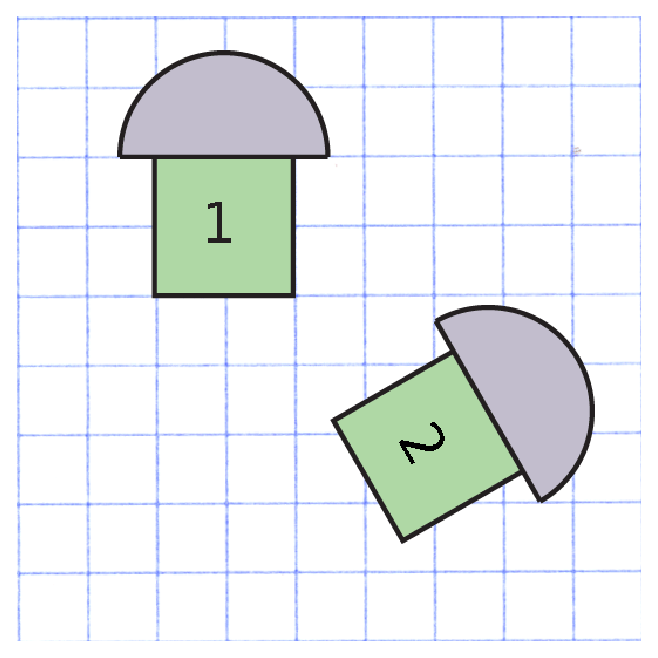
\includegraphics[width=4.7cm]{champi_rotation}
  \end{minipage} \hfill%
  \begin{minipage}[c]{0.58\linewidth}
Alice sait que la figure 2 a été obtenue après une rotation de la figure 1. \\[0.5em]
Pascal aimerait savoir où se trouve le centre de la rotation ainsi que l'angle de rotation. \\[0.5em]
Aline propose de tracer les médiatrices des segments reliant les sommets de la figure 1 aux sommets correspondants de la figure 2.
  \end{minipage} \\
\begin{enumerate}
 \item Recopie la figure puis effectue ce qu'Aline propose.
 \item Que remarques-tu ?
 \item Détermine où se trouve le centre ainsi que l'angle de la rotation qui permet de passer de la figure 1 à la figure 2.
 \end{enumerate}
\end{partie}

\end{activite}

%%%%%%%%%%%%%%%%%%%%%%%%%%%%%%%%%%%%%%%%%%%%%%%%%%%%%%%%%%%%%%%%%%%%%%
